\documentclass{cheatsheet}

\usepackage{bm}

\doctitle{Chemistry Cheatsheet}
\author{Noa Sendlhofer \& Christian Leser \\ nsendlhofer \& cleser}

\begin{document}
\section{1. Basics} %Noa
	\subsection{1.1 Unit conversions}
	\begin{itemize}
		\itemsep0em
		\raggedright
  		\item \textbf{Energy:} $1eV=1.602\cdot 10^{-19}J$,    $1cal=4.18J$
    	\item \textbf{Pressure:} $P = \frac{F}{A} = \rho \cdot h \cdot g$\\ $1 \textrm{atm} = 760mm \; \textrm{Hg} = 760 \textrm{torr} = 101'325 \textrm{Pa} = 1.01325 \textrm{bar}$\\ Manometer: $P = P_{atm}\pm \rho g h$
    	\item \textbf{Force:} $F = m \cdot g, \; m = \rho \cdot V$
		\item \textbf{Amount of substance:} $1 \textrm{mol} = 6.022\cdot 10^{23} \textrm{(Avogadro)}$
    	\item \textbf{Length:} $1\text{Å}=10^{-10}m$
    	\item \textbf{STP; } $0\tccentigrade = 273.15K, \; 1atm; \; V_m = 22.41L$
	\end{itemize}

\subsection{1.2 General}
    \begin{itemize}
		\itemsep0em
        \item \textbf{Kinetic energy:} $E_{kin} = \frac{1}{2} \cdot m \cdot v^2$
        \item \textbf{Potential energy:} $E_{pot} = m \cdot g \cdot \Delta h$
        \item \textbf{electrostatic:} $E_{el}=\frac{\kappa Q_1Q_2}{d^2}$\quad $\kappa = \frac{1}{4\pi \epsilon_0}$
        \item \textbf{Photon energy: } $E_\gamma = h\cdot f = \frac{h\cdot c}{\lambda}$
        \item \textbf{De Broglie wavelength: } $\lambda = \frac{h}{m\cdot v}$
    \end{itemize}
    	
\subsection{1.3 Trends in the periodic table of elements}
	\begin{itemize}
		\itemsep0em
    	\item \textbf{Ionisation energy: }The ionization energy is the quantity of energy that an isolated, gaseous atom in the ground electronic state must absorb to discharge an electron, resulting in a cation.
    	\item \textbf{Electron affinity: }Electron affinity is defined as the change in energy (in kJ/mole) of a neutral atom (in the gaseous phase) when an electron is added to the atom to form a negative ion.
    	\item \textbf{Electronnegativity:} Electronegativity is a measure of an atom's ability to attract shared electrons to itself.
	\end{itemize}
	\centerline{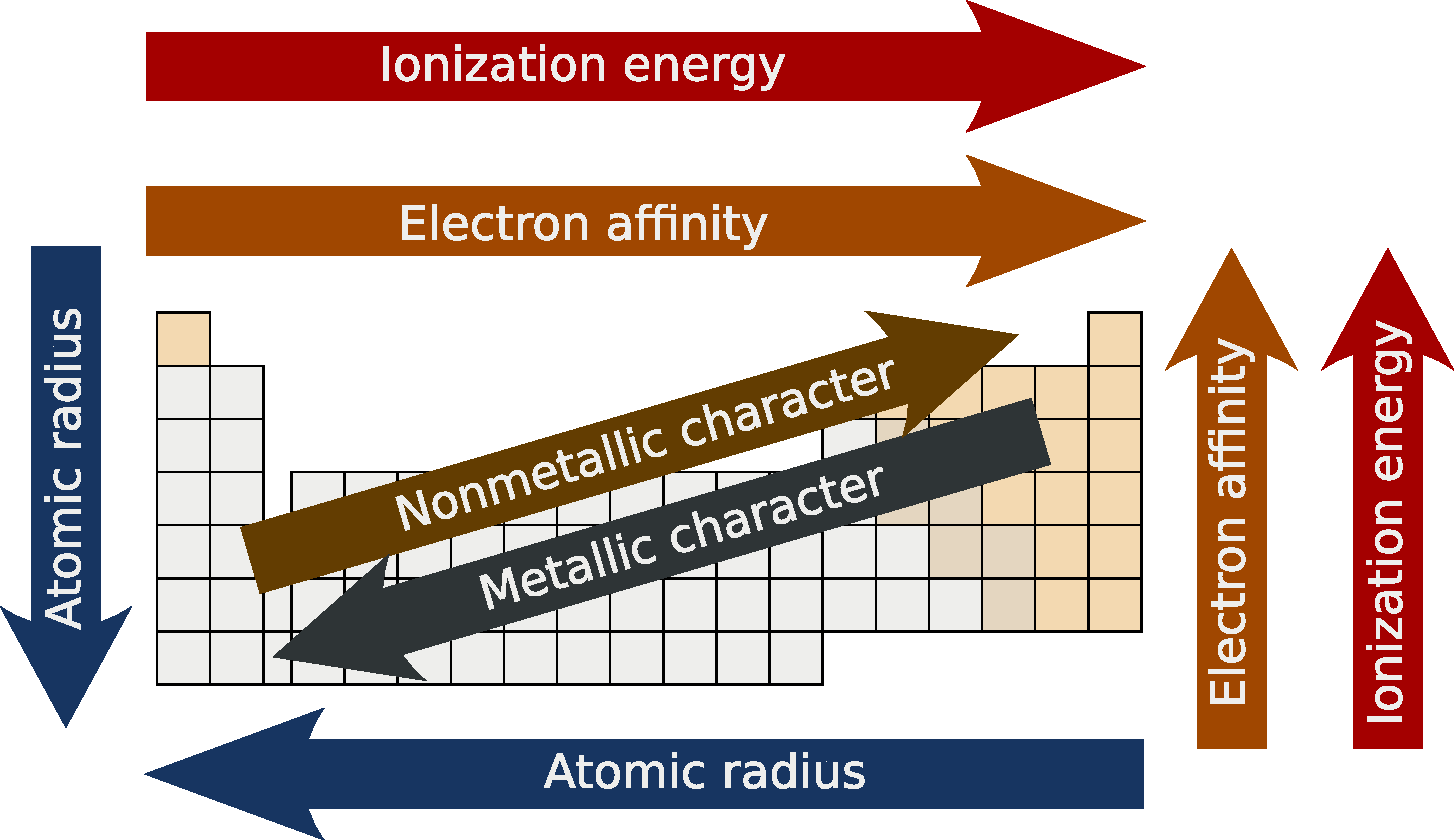
\includegraphics[width=0.65\linewidth]{src/1_Basics/Periodic_trends.pdf}}
	\vspace*{0.5em}
\vfill \null \columnbreak

\section{2. Atoms} %Christian
	\subsection{2.1 Quantum mechanics}
	\subsection{2.1 Quantum mechanics}
    \begin{scriptsize}
        \begin{tabular}{c c}
            Atomic mass = total mass & Atomic weight = average atomic mass (isotopes)\\
            Atomic number = \#protons & mass number = \#protons + \#neutrons
        \end{tabular}
    \end{scriptsize}
        \vspace*{0.0em}
        
        Heisenbergs uncertainty principle $\Delta x \cdot \Delta p \geq \frac{h}{4 \cdot \pi}$ Due to duality of electrons (acting like waves and elementary entities at the same time), impossible to exactly describe position and momentum simultaneously.\\
        \textbf{Effective nuclear charge (approx.):}   $Z_{eff} = Z-S$\\
        $Z$ = \#protons, $S$ = \#$e^-$ on all full shells
        \vspace{1mm}\\
        In periodic table: $Z_{eff}$ increases from left to right $\rightarrow$ electrons are more attracted and hence atomic radius is smaller, the further right in the periodic table. ($e^-$ repulsion vs. nuclear charge)
        \vspace*{0.0em}
	\subsection{2.2 Orbitals}
	\subsection{2.2 Orbitals}
  \begin{minipage}{0.99\linewidth}
    \begin{minipage}{0.33\linewidth}
      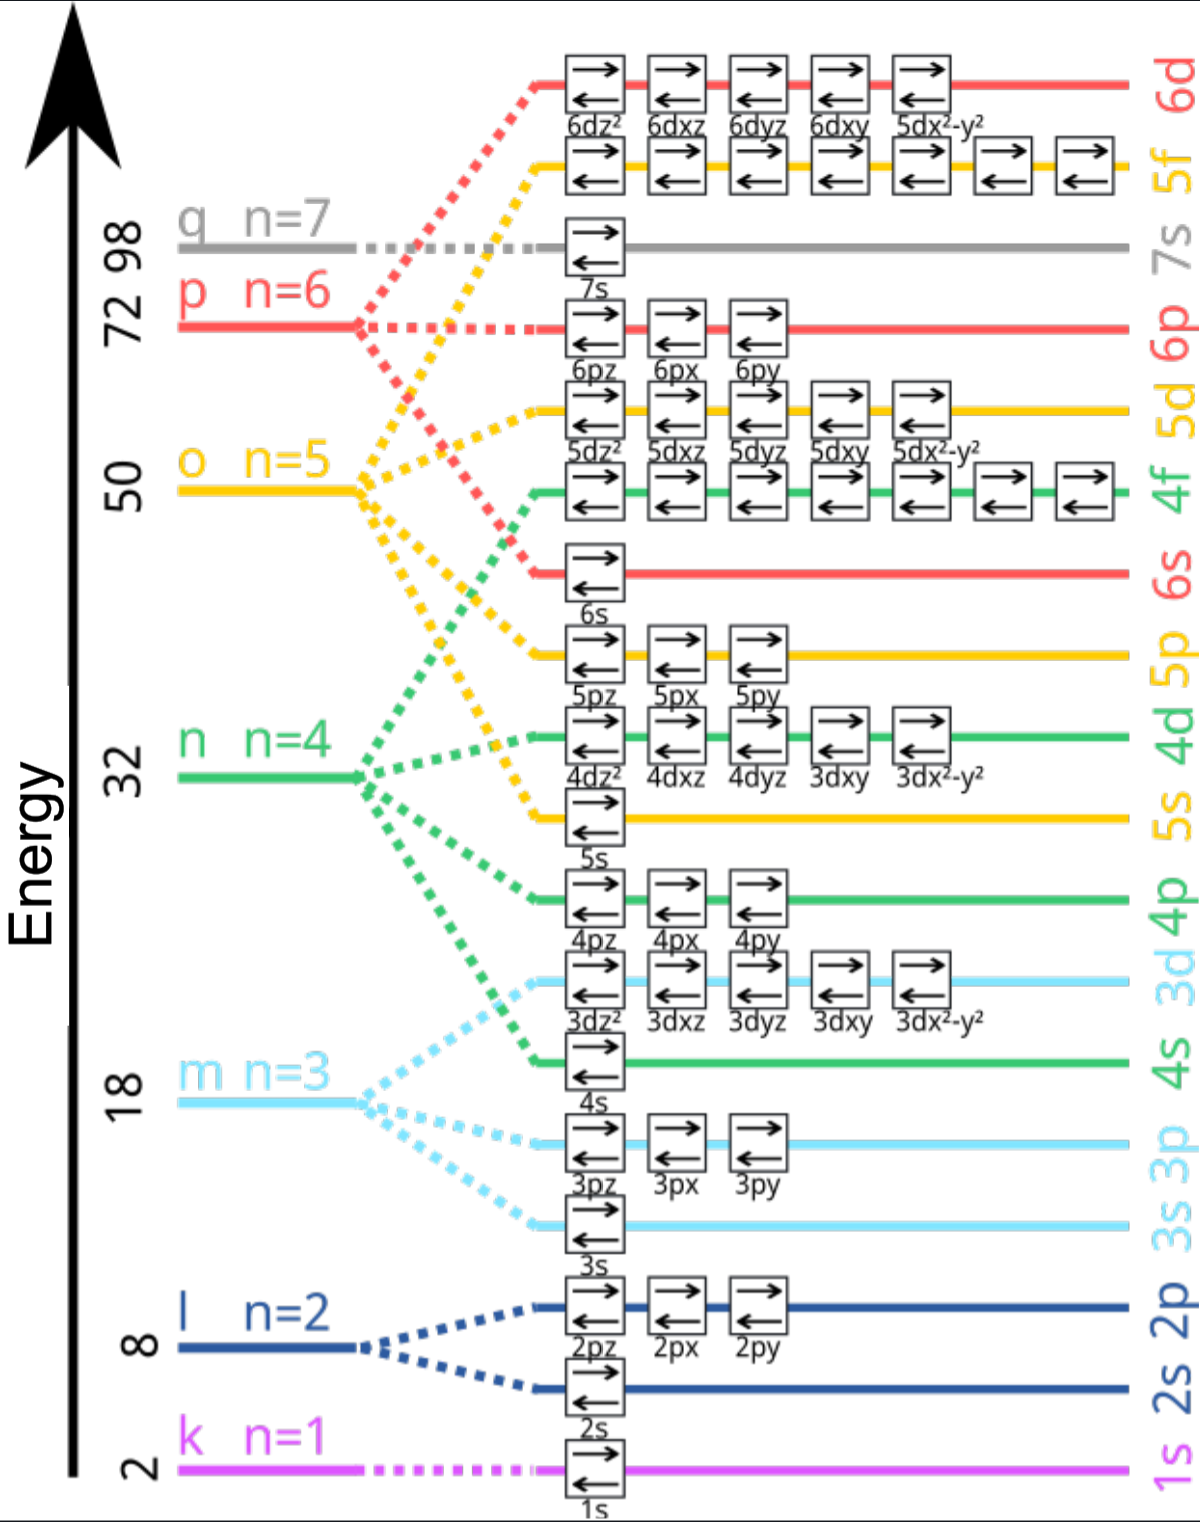
\includegraphics[width = 2.3cm]{src/2_Atoms/images/Energieniveau.png}
    \end{minipage}
    \begin{minipage}{0.52\linewidth}
      \begin{scriptsize}
        \begin{center}
            \begin{tabular}{|p{0.3mm}|c|p{0.07\textwidth}|c|c|}
                \multicolumn{1}{p{0.3mm}}{n} & \multicolumn{1}{c}{l} & \multicolumn{1}{p{0.07\textwidth}}{\rotatebox{90}{\pbox{1.5cm}{subshell\\ designation}}} & \multicolumn{1}{c}{$m_i$} & \multicolumn{1}{c}{$m_s$} \\ [0.5ex]
                \hline
                1 & 0, s & 1s                                  & 0                      & $\pm 1/2$ \\ 
                \hline
                2 & 0, s & 2s                                  & 0                      & $\pm 1/2$ \\
                  & 1, p & 2p                                  & 1, 0, -1               & $\pm 1/2$ \\
                \hline
                3 & 0, s & 3s                                  & 0                      & $\pm 1/2$ \\
                  & 1, p & 3p                                  & 1, 0, -1               & $\pm 1/2$ \\
                  & 2, d & 3d                                  & 2, 1, 0, -1, -2        & $\pm 1/2$ \\
                \hline
                4 & 0, s & 4s                                  & 0                      & $\pm 1/2$ \\
                  & 1, p & 4p                                  & 1, 0, -1               & $\pm 1/2$ \\
                  & 2, d & 4d                                  & 2, 1, 0, -1, -2        & $\pm 1/2$ \\
                  & 3, f & 4f                                  & 3, 2, 1, 0, -1, -2, -3 & $\pm 1/2$ \\
                \hline
            \end{tabular}
        \end{center}
        \end{scriptsize}
    \end{minipage}
  \end{minipage}
        
    \begin{itemize}
        \itemsep0em
        \item \textbf{n}: principal quantum number $\rightarrow$ size of orbital
        \item \textbf{l}: angular quantum number $\rightarrow$ shape of orbital
        \item $\boldsymbol{m_l}$: magnetic quantum number $\rightarrow$ orientation of orbital
        \item $\boldsymbol{m_s}$: spin quantum number
    \end{itemize}
    \vspace*{-0.9em}
    
    \begin{minipage}{0.99\linewidth}
      \begin{minipage}{0.45\linewidth}
        \centerline{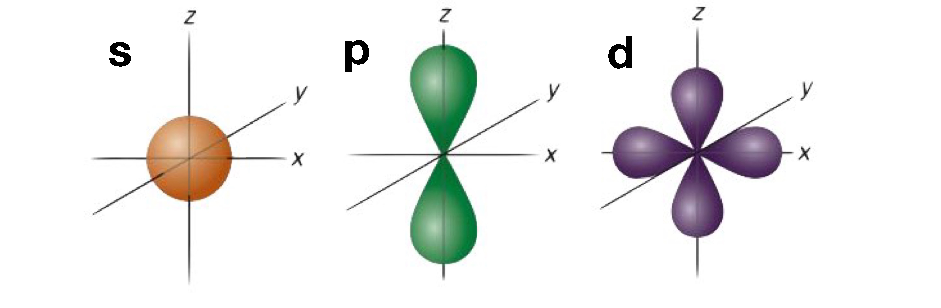
\includegraphics[width=35mm]{src/2_Atoms/images/orbital_shapes.pdf}}
      \end{minipage}
      \begin{minipage}{0.54\linewidth}
        \centerline{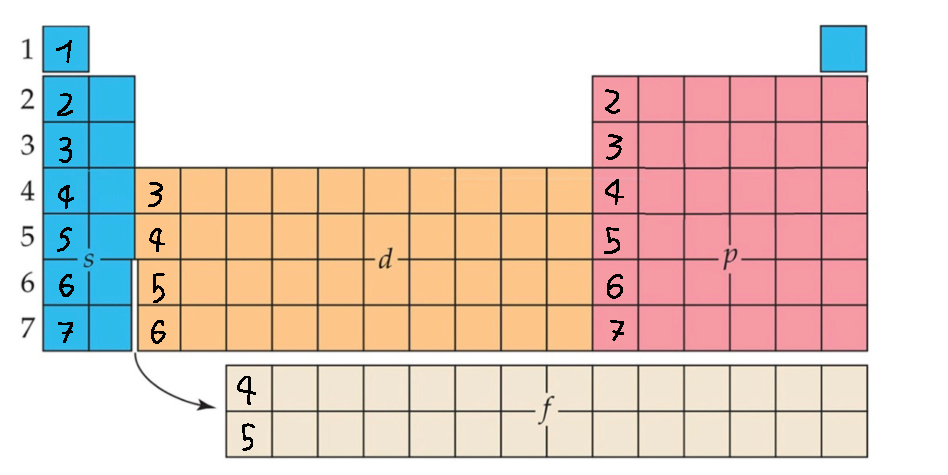
\includegraphics[width=43mm]{src/2_Atoms/images/pse_electron_config.pdf}}
      \end{minipage}
    \end{minipage}
    
    Pauli Exclusion: Each electron has unique set of quantum numbers\\
    Hund's rule: \textbf{Every} orbital in sublevel is first singly occupied\\
    Energy of Hydrogen $e^-$: $E_n = -\frac{hcR_H}{n^2}$, $R_h = 1.097 \cdot 10^7 m^{-1}$\\
    Excitement from shell $n_1$ to $n_2$: $E_H = hcR_H (\frac{1}{n_1^2} - \frac{1}{n_2^2})$

\section{3. Chemical bondings} %Christian
	\subsection{3.1 Covalent bondings}
	\subsection{3.1 Covalent bondings}
    Two atoms share electron pairs\\
    \textbf{octet rule:} Atom tries to acquire noble state (2 valence electrons for H and He, 8 valence electrons for all other)\\
    \textbf{exceptions:} 
    \begin{itemize}
        \itemsep0em
        \item Odd electrons
        \item Less / more than 8 VE's on central atom
    \end{itemize}
	\subsection{3.2 Polarity and Dipole moment}
	\subsection{3.2 Polarity and Dipole moment} 
    $\Delta EN>0.5$: polar bonding, density of $e^-$ higher at $\delta^-$ atom.
        If molecular structure leads to  $\rightarrow$ dipole moment exists.
        \begin{center}
            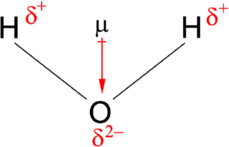
\includegraphics[width=0.3\linewidth]{src/3_Chemical_bondings/images/dipole_moment.png}
        \end{center}
	\subsection{3.3 Formal charges}
	results if new bondings are formed to satisfy octet rule, ignores electronegativity\\
\textbf{Determine formal charge in Molecule:}
\begin{itemize}
    \itemsep0em
    \item split all bondings in middle
    \item atoms formal charge = VE if unpaired $- e^-$ of that atom after splitting bondings
    \item effective charge of molecule = sum of formal charges
\end{itemize}

	\subsection{3.4 Bonding strength and length}
	\begin{tabular}{c c}
    \textbf{length:} $\equiv < = < -$ & \textbf{strength:} $- < = < \equiv$\\
\end{tabular}\\
\textbf{Most stable molecule:}
\begin{itemize}
    \itemsep0em
    \item least formal charges.
    \item if formal charges necessary: option with the smallest effective charge of molecule
    \item negative formal charge on electronegative atom
\end{itemize}
	\subsection{3.5 Lewis structure}
	\begin{itemize}
    \itemsep0em
    \item Write symbols and connect with single bonds
    \item Complete ocets around non-central atoms
    \item Place remaining VE around central atom
    \item Try multiple bonds if central atom does not have octet
    \item if multiple lewis structures possible: choose most stable according to formal charge
    
\end{itemize}
	\subsection{3.6 Ionic bonding}
	Electrons transfered from atoms with lower EN to atoms with higher EN $\rightarrow$ cations (+) and anions (-).\ electrostatic attraction. $\Delta EN > 1.7 \rightarrow$ ionic bonding\\
molar lattice energy $\Delta U$ = Energy set free when grid of ions is formed e.g.\ salt
	\subsection{3.7 Metallic bonding}
	\begin{minipage}{25mm}
    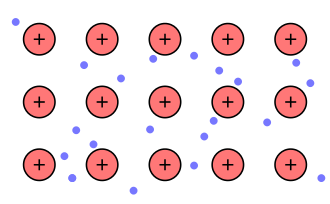
\includegraphics[width=2.5cm]{src/3_Chemical_bondings/images/Metallische Bindung.png}
\end{minipage}
\begin{minipage}{42mm}
    Positiv geladene Kerne umgeben von einer negativ geladenen Elektronenwolke. Metalle haben
    Defizit an VE $\rightarrow$ zu wenig VE, um Kovalente Bindung einzugehen. Frei bewegliche Ladungen 
    (Elektronenwolke) sind Ursache für gute Strom- und Wärmeleitfähigkeit.
\end{minipage}
	

\section{4. Molecular models}
	\input{src/4_Molecular_models/4_molecular_models}

\section{5. State of matter} %Noa
	\subsection{5.1 Intermolecular forces}
    \begin{enumerate}
        \item \textbf{Van-der-Waals interactions} (weak)
            \begin{enumerate}
                \item \textbf{Dipol-Dipol} \\
                    Sum of all dipole moments from polar bonds in molecule. (molecular dipole) ($\Delta EN>0.5$)
                \item \textbf{Dispersion} \\
                    Temporary fluctuations of the electrons can cause an induced dipole.
                    \textbf{These forces always exist}. Force increases with molecule size and also affected by molecular shape.
            \end{enumerate}
        \item \textbf{Ion-Dipole Interactions} (strong)\\
            Very important for solutions. Ions solvated by polar liquid.
        \item \textbf{Hydrogen bonding} (strong)\\
            One type of dipole-dipole interaction. N, O, F are very electronegativ $\Rightarrow$ very polar bonds with H.
    \end{enumerate}
    \vspace*{-0.5em}
    \centerline{
        \parbox[t]{1.5cm}{
        \centering
        Ion-Dipole\\$>$ 50kJ/mol}%
        \bm{$>$}
        \parbox[t]{1.5cm}{
        \centering
        H-Bonding\\$\sim$ 25kJ/mol}%
        \bm{$>$}
        \parbox[t]{3cm}{
        \centering
        Dipole-Dipole $\approx$ Dispersion\\$\sim$ 50kJ/mol}%
    }
	\subsection{5.2 Fluids}
    \textbf{Colligative Properties: }Changes depend on amount of solute added, but not which solute.
    $$
    \text{Clausius-Clapeyron} \left\{
        \begin{array}{ll}
            \ln(P_{vap}) = - \frac{\Delta H_{vap}}{RT} + C\\
            \ln(\frac{P_1}{P_2}) = \frac{\Delta H_{vap}}{R} \left( \frac{1}{T_2} - \frac{1}{T_1} \right)
        \end{array}
        \right.
    $$\\*

    % \begin{align*}
    %     \ln(P_{vap}) =& - \frac{\Delta H_{vap}}{RT} + C\\
    %     \ln(\frac{P_1}{P_2}) =& \frac{\Delta H_{vap}}{R} \left( \frac{1}{T_2} - \frac{1}{T_1} \right)
    % \end{align*}

    \textbf{Boiling-Point Elevation:}
    \begin{align*}
        \Delta T_b & = T_b (\textrm{solution}) - T_b (\textrm{solvent}) = iK_b m\\
        m & = \text{molality of solute}\\
        K_b & = \text{molal bp elevation constant (solvent)}\\
        i & = \text{van't Hoff factor}\\
        & = 1 \text{ for non-electrolytes}\\
        & = \text{Number of ions produced for electrolytes.\ e.g 2 for NaCl}
    \end{align*}
    
    \textbf{Vapor-Pressure Lowering: }
        \mathbox{
            P_\text{vap}^\text{sol} = X_\text{solvent} * P_\text{vap}^\text{pure}
        }
    
        Raoult's law $-$ Solution is an ideal solution. All intermolecular interactions are identical.\\

    \textbf{Freezing-Point Depression: }
        \begin{align*}
            \Delta T_f & = T_f (solution) - T_f (solvent) = -iK_{f}m\\
            m & = \text{molality of solute} = (\textrm{moles of solute}) / (\textrm{kg of solvent})\\
            K_f & = \text{molal fp depression constant (solvent)}\\
            i & = \text{van't Hoff factor}
        \end{align*}
	\subsection{5.3 Ideal Gas}
    \begin{itemize}
        \item Assumptions of IGL:
        \begin{itemize}
            \item Gas molecules don't occupy much of total volume.
            \item Gas molecules don't interact.
        \end{itemize}
        \item Ideal Gas Law: $pV = nRT=N kT$
        \item $p\left[Pa\right], V\left[m^3\right], n\left[\text{num of moles}\right], R\left[\frac{J}{mol*K}\right], T\left[K\right]$
        \item Density $\rho = M\frac{n}{V}=M\frac{p}{RT}$
    \end{itemize}
    \subsubsection{Partial pressure:}
        \mathbox{
            p_i=n_i\cdot\frac{RT}{V} \text{ total pressure} =\Sigma \text{ of all partial pressures.}
        }
	\subsection{5.4 Osmotic pressure}
    Pressure needed to counteract osmotic flow.
    \mathbox{
        \Pi = i\left(\frac{n}{V}\right)RT=iMRT
    }


\section{6. Thermodynamics}
	\input{src/6_Thermodynamics/6_thermodynamics}

\section{7. Kinetics}
	\input{src/7_Kinetics/7_kinetics}

\section{8. Acids and Bases}
	\input{src/8_Acids_and_Bases/8_acids_and_bases}

\section{9. Redox reactions}
	\input{src/9_Redox_rxns/9_redox_rxns}

\end{document}